% IF YOU CAN SEE THIS GO CONTRIBUTE >:(

\documentclass[letterpaper, 8pt]{extarticle}
\usepackage{amssymb,amsmath,amsthm,amsfonts}
\usepackage{multicol,multirow}
\usepackage{calc}
\usepackage{ifthen}
\usepackage[landscape]{geometry}
\usepackage[colorlinks=true,citecolor=blue,linkcolor=blue]{hyperref}

\usepackage{booktabs}
\usepackage{ulem}
\usepackage{enumitem}
\usepackage{tabulary}
\usepackage{graphicx}
\usepackage{siunitx}
\usepackage{tikz}
\usepackage{derivative}
\usepackage{svg}
\usepackage{listings}
\usepackage{setspace}
\usepackage{listings}
\usepackage{xcolor}
\usepackage{courier}
\usepackage{syntax}
\usepackage{mathpartir}

% minimal line spacing
\setstretch{0.1}

% set borders (experimentally determined to minimize cutoff and maximize space on school printers)
\geometry{top=.25in,left=.25in,right=.25in,bottom=.35in}

% make figures work better in multicol
\newenvironment{Figure}
{\par\medskip\noindent\minipage}
{\endminipage\par\medskip}

\pagestyle{empty} % clear page

% rewrite section commands to be smaller
\makeatletter
\renewcommand{\section}{\@startsection{section}{1}{0mm}%
                                {-1explus -.5ex minus -.2ex}%
                                {0.5ex plus .2ex}%x
                                {\normalfont\normalsize\bfseries}}
\renewcommand{\subsection}{\@startsection{subsection}{2}{0mm}%
                                {-1explus -.5ex minus -.2ex}%
                                {0.5ex plus .2ex}%
                                {\normalfont\small\bfseries}}
\renewcommand{\subsubsection}{\@startsection{subsubsection}{3}{0mm}%
                                {-1ex plus -.5ex minus -.2ex}%
                                {1ex plus .2ex}%
                                {\normalfont\tiny\bfseries}}
\makeatother
\setcounter{secnumdepth}{0} % disable section numbering

% disable indenting
\setlength{\parindent}{0pt}
\setlength{\parskip}{0pt plus 0.5ex}

% Custom siunitx defs
\DeclareSIUnit\noop{\relax}
\NewDocumentCommand\prefixvalue{m}{%
\qty[prefix-mode=extract-exponent,print-unity-mantissa=false]{1}{#1\noop}
}

% Shorthand definitions
\newcommand{\To}{\Rightarrow}
\newcommand{\ttt}{\texttt}
\newcommand{\ra}{\rightarrow}

% condense itemize & enumerate
\let\olditemize=\itemize \let\endolditemize=\enditemize \renewenvironment{itemize}{\olditemize \itemsep0em}{\endolditemize}
\let\oldenumerate=\enumerate \let\endoldenumerate=\endenumerate \renewenvironment{enumerate}{\oldenumerate \itemsep0em}{\endoldenumerate}
\setlist[itemize]{noitemsep, topsep=0pt, leftmargin=*}
\setlist[enumerate]{noitemsep, topsep=0pt, leftmargin=*}

\title{3MI3}

\begin{document}
\raggedright
\tiny

% make listings look nicer
\lstset{
    tabsize = 2, %% set tab space width
    showstringspaces = false, %% prevent space marking in strings, string is defined as the text that is generally printed directly to the console
    basicstyle = \tiny\ttfamily, %% set listing font and size
    breaklines = true, %% enable line breaking
    numberstyle = \tiny,
    postbreak = \mbox{\textcolor{red}{\(\hookrightarrow\)}\space}
}

\begin{center}
    {\textbf{3MI3 Final -- Year of the Rabbit Edition}} \\
\end{center}
% set column spacing rules
\setlength{\premulticols}{1pt}
\setlength{\postmulticols}{1pt}
\setlength{\multicolsep}{1pt}
\setlength{\columnsep}{2pt}
\begin{multicols*}{4}
    \section{Programming languages}
    \subsection{Important languages}
    \textbf{Fortran} -- First lang w/ a compiler, syntax is whatever the compiler accepts, no formal standards set.
    \textbf{Lisp} -- Computing abstract / symbolic stuff, dynamic scope for variables.
    \textbf{COBOL} -- Used for ``business'' programming, verbose and made to read like English, good layout capabilities.
    \textbf{Algol 60} -- First language with a standard (BNF invented for this), designed by committee.
    \textbf{ML} -- Abstract data types, hides details about types from programmer, can't lie to compiler, tradeoff of more debugging for less hassle down the line.

    \subsection{Esoteric languages}
    Esolangs are programming languages designed to experiment with weird ideas, made intentionally hard to program in, or as a joke, rather than practical use.
    Esolangs are known for breaking modern coding conventions to possible innovate with new ideas.
    Some examples of esolangs are Shakespeare, Befunge (2D text syntax), LOLCODE, Malbolge (designed to be unwritable - `crazy operation', base-three arithmetic, and self-altering code), INTERCAL (satire of programming languages and new notation), Brainfuck (minimal, unreadable turing machine simulator), and PIET (syntax as blocks of colour in an image).

    \section{Syntax}
    How a programming language ``looks''.
    Often a string, but can be a picture (Monet), or a grid of cells (Excel).
    \subsection{BNF}
    Formal specification of string-based syntaxes.
    \begin{grammar}
        <e> ::= x
        \alt \(\lambda x <e>\)
        \alt <e> <e>
        \alt (<e>)
    \end{grammar}

    \section{Dynamic Semantics}
    % Small-step semantics
    % -> Lambda calculus - Call-by-name vs Call-by-value
    % domain-specific languages
    % shallow vs deep vs tagless embeddings

    \subsection{Evaluation Strategies}

    Can't evaluate anything under a lambda in both of the below strategies.
    \subsubsection{Full Beta-Reduction:} beta-reduce in any order: non-deterministic.
    \subsubsection{Normal Order:} reduce the leftmost, outermost expression until no more expressions.
    \subsubsection{Call by Name} --
    Evaluate function calls without evaluating arguments. Stop when the outermost term is a lambda.
    % idk put the rules or an example here

    % TODO: if we run out of space delete this and replace it with an explanation
    \(\inferrule{e_1 \to e_1'}{e_1 e_2 \to e_1' e_2}\)
    \(\inferrule{ }{(\lambda x.e_1)e_2 \to e_1[e_2/x]}\)
    \(\inferrule{ }{\operatorname{fst}(e_2, e_2) \to e_2}\)
    \(\inferrule{ }{\operatorname{snd}(e_1, e_2) \to e_2}\)
    \(\inferrule{e_1 \to e_1'}{\operatorname{and} e_1 e_2 \to \operatorname{and} e_1' e_2}\)
    \(\inferrule{ }{\operatorname{and}\operatorname{true} e_2 \to e_2}\)
    \(\inferrule{ }{\operatorname{and}\operatorname{false} e_2 \to \operatorname{false}}\)
    \(\inferrule{e_1 \to e_1'}{\operatorname{if} e_1 \operatorname{then} e_2 \operatorname{else} e_3 \to \operatorname{if} e_1' \operatorname{then} e_2 \operatorname{else} e_3}\)
    \(\inferrule{ }{\operatorname{if}\operatorname{true}\operatorname{then} e_2 \operatorname{else} e_3 \to e_2}\)
    \(\inferrule{ }{\operatorname{if}\operatorname{false}\operatorname{then} e_2 \operatorname{else} e_3 \to e_3}\)
    \(\inferrule{ }{\operatorname{let} x = e_1 \operatorname{in} e_2 \to e_2[e_1/x]}\)

    \subsubsection{Call by Value} --
    Evaluate arguments to function calls before evaluating the function call itself. Stop when the outermost term is a lambda. This is the evaluation strategy most languages adopt.

    \(\inferrule{e_1 \to e_1'}{e_1 e_2 \to e_1' e_2}\)
    \(\inferrule{e_2 \to e_2'}{v_1 e_2 \to v_1 e_2'}\)
    \(\inferrule{ }{(\lambda x.e_1) v_2 \to e_1[v_2/x]}\)
    \(\inferrule{e_1 \to e_1'}{(e_1, e_2) \to (e_1', e_2)}\)
    \(\inferrule{e_2 \to e_2'}{(v_1, e_2) \to (v_1, e_2')}\)
    \(\inferrule{ }{\operatorname{fst} (v_1, v_2) \to v_1}\)
    \(\inferrule{ }{\operatorname{snd} (v_1, v_2) \to v_2}\)
    \(\inferrule{e_1 \to e_1'}{\operatorname{and} e_1 e_2 \to \operatorname{and} e_1' e_2}\)
    \(\inferrule{ }{\operatorname{and}\operatorname{true} e_2 \to e_2}\)
    \(\inferrule{ }{\operatorname{and}\operatorname{false} e_2 \to \operatorname{false}}\)
    \(\inferrule{e_1 \to e_1'}{\operatorname{if} e_1 \operatorname{then} e_2 \operatorname{else} e_3 \to \operatorname{if} e_1' \operatorname{then} e_2 \operatorname{else} e_3}\)
    \(\inferrule{ }{\operatorname{if}\operatorname{true}\operatorname{then} e_2 \operatorname{else} e_3 \to e_2}\)
    \(\inferrule{ }{\operatorname{if}\operatorname{false}\operatorname{then} e_2 \operatorname{else} e_3 \to e_3}\)
    \(\inferrule{e_1 \to e_1'}{\operatorname{let} x = e_1 \operatorname{in} e_2 \to \operatorname{let} x = e_1' \operatorname{in} e_2}\)
    \(\inferrule{ }{\operatorname{let} x = v_1 \operatorname{in} e_2 \to e_2[v_1/x]}\)

    % somebody please fix the formatting on this
    % \textbf{Call by Value rules for pairs only}
    % $\begin{array}{ccc}
    %     \begin{array}{c}
    %     e_{1}\rightarrow e_{1}'\\
    %     \hline
    %     (e_{1}, e_{2}) \rightarrow (e_{1}', e_{2})
    %     \end{array}\\
    %     &
    %     \begin{array}{c}
    %     e_{2}\rightarrow e_{2}'\\
    %     \hline
    %     (v_{1}, e_{2}) \rightarrow (v_{1}, e_{2}')
    %     \end{array}\\
    %     &
    %     \begin{array}{c}
    %     e\rightarrow e'\\
    %     \hline
    %     \mathrm{fst}\ e \rightarrow \mathrm{snd}\ e'
    %     \end{array}\\
    %     \\
    %     \begin{array}{c}
    %     e\rightarrow e'\\
    %     \hline
    %     \mathrm{snd}\ e\rightarrow \mathrm{snd}\ e'
    %     \end{array}\\
    %     &
    %     \begin{array}{c}
    %     \\
    %     \hline
    %     \mathrm{fst}\ (v_{1}, v_{2}) \rightarrow v_1
    %     \end{array}\\
    %     &
    %     \begin{array}{c}
    %     \\
    %     \hline
    %     \mathrm{snd}\ (v_{1}, v_{2}) \rightarrow v_2
    %     \end{array}
    %     \end{array}$

    % add if u want
    % \section{Typing Rules}

    \subsection{Church Encodings}

    \subsubsection{Booleans}
    tru = $\lambda t. \lambda f. t $\\
    fls = $\lambda t. \lambda. f. f $\\
    and = $\lambda b. \lambda c. b c \ \text{fls}$\\
    or = $\lambda b. \lambda c. b \ \text{tru} \  c$ %correct this if wrong idk if this is right
    not = $\lambda p. p \ \text{fls}\ \text{tru}$

    \subsubsection{Numerals}
    0 = $\lambda s. \lambda z. z$\\
    1 = $\lambda s. \lambda z. s z$\\
    2 = $\lambda s. \lambda z. s (s z)$
    plus = $\lambda m.\lambda n.\lambda f.\lambda x. m\ f\ (n\ f\ x)$ \\
    succ = $\lambda n.\lambda f.\lambda x. f\ (n\ f\ x)$\\
    mult = $\lambda m.\lambda n.\lambda f.\lambda x.m\ (n\ f)\ x$\\
    exp = $\lambda m.\lambda n. n\ m$\\
    pred = $\lambda n.\lambda f.\lambda x. n\ (\lambda g.\lambda h. h\ (g\ f))\ (\lambda u. x)\ (\lambda u. u)$\\
    pred = $\lambda m. fst (m ss zz)$ where $ss = \lambda p. pair (snd p) (plus c_1 (snd p))$ and
    $zz = pair c_0 c_0$\\
    minus = $\lambda m.\lambda n. (n \ \text{pred})\ m$\\
    iszero = $(\text{minus}\ n\ m)$\\
    iszero = $\lambda m.m (\lambda x.\ \text{fls}) \text{tru}$\\

    \subsubsection{Pairs}
    pair = $\lambda x.\lambda y.\lambda z.z\,x\,y$\\
    fst = $\lambda p.p (\lambda x.\lambda y.x)$\\
    snd = $\lambda p.p (\lambda x.\lambda y.y)$

    \subsubsection{Either} % someone check if these are wrong
    left = $\lambda a. \lambda l. \lambda r. l a$\\
    right = $\lambda b. \lambda l. \lambda r. r b$

    \subsubsection{Lists}
    nil = $\lambda c.\lambda n.n$\\
    cons = $\lambda h.\lambda t.\lambda c.\lambda n.c\,h\,(t\,c\,n)$\\
    isnil = $\lambda l. l (\lambda h. \lambda t. \ \text{fls}) \ \text{tru}$\\
    head = $\lambda l. l (\lambda h. \lambda t. h) \ \text{fls}$\\
    tail = $\lambda l. \lambda c. \lambda n. l (\lambda h. \lambda t. \lambda g. g h (t c)) (\lambda t. n) (\lambda h. \lambda t. t)$\\

    % credit to milenb17#9439 on Discord
    \subsubsection{Trees}
    leaf = \(\lambda x.\lambda b.\lambda l.l ,x\)\\
    branch = \(\lambda x.\lambda y.\lambda b.\lambda l. ,b ,(x, l, b) ,(y, l, b)\)

    \subsection{Domain Specific Languages (DSLs)}
    \subsubsection{Shallow}
    Implement the DSL as functions.
    Ex. for pic DSL, stuff is given as functions.
    Easy to add new functions,
    but can suck if you want to extend to more interpretations since you can't reuse functions.
    Pros:
    \begin{itemize}
        \item{easy extensibility of terms}
        \item{Has nice syntax due to being programmed in an established language}
        \item{piggyback on host language's type system (pro in some cases)}
    \end{itemize}
    Cons:
    \begin{itemize}
        \item{no reuse of ASTs}
        \item{Hard to re-interpret terms with other meanings (e.g. hard to change format of a picture)}
        \item{things are immediately evaluated}
        \item{piggyback on host language's type system (con in some cases), e.g. if you want
              to move your dsl to another language}
        \item{Cannot easily perform program transformations (e.g. optimizations)}
    \end{itemize}
    \subsubsection{Deep}
    Datatype to represent syntax.
    Can easily write new interpretation functions.
    But annoying to add new operations because all interpretations need to be extended.
    Pros:
    \begin{itemize}
        \item{easy reuse of programs written in the DSL}
        \item{custom validity system}
        \item{simulatable}
        \item{domain-specific interpretations, e.g. tool creation, analysis, re-writing, optimization passes, etc.}
        \item{Can easily perform program transformations (e.g. optimizations)}
    \end{itemize}
    Cons:
    \begin{itemize}
        \item{Ugly syntax}
        \item{extra tag i.e. the DSL is a little less efficient}
        \item{term set is typically not 'open'}
              \begin{itemize}
                  \item{we can't easily extend a language without recompilation
                        and defining interpreation of new terms for all previously
                        defined operators}
                  \item{expression problem (? related to above?)}
              \end{itemize}
    \end{itemize}
    \subsubsection{Tagless}
    Best of shallow and deep.
    The language is the interpretation.
    If we want to add a new operation we can easily add a new class that extends the original.
    To create a new interpretation just create an instance of the class.
    Pros:
    \begin{itemize}
        \item{Both of the pros from shallow and deep embeds}
        \item{Programming against an abstract interface is nice}
    \end{itemize}
    Cons:
    \begin{itemize}
        \item{Speed: the compiler does not know what you are working against with an abstract
              interface so compiler optimizations might not work properly}
    \end{itemize}

    \section{Static Semantics (Typing)}
    % types
    % Progress rule (always be able to make a step towards the value)
    % (for every well-typed program, either I can make a step, or e is a value)
    % Preservation rule (if a term is well-typed, and we evaluate it once under
    % single-step operational semantics, the resulting term is also well typed.)
    \textbf{Type safety} is an assurance that computations do not lead to mismatched types in other computations — program execution does not lead to ill-defined states.
    A \textbf{type system} consists of two pieces; judgements and inference rules. A judgement is some property that the type system lets us show; for instance, we might have a judgement that asserts that some term x has type A. The inference rules allow us to actually prove that some judgement holds. For instance, this is how one might prove that (true, false) has type Bool × Bool.
    DSLs are particularly neat because they allow for domain-specific: analysis, validation, interpretation, optimization, tooling, etc.

    \subsection{Progress}
    Definition: a well-typed term is either a value or, or
    may be evaluated once under single-step operational semantics. That is, a
    well-typed term is not stuck.
    \subsection{Preservation}
    Definition: if a term is well-typed, and we evaluate it
    once under single-step operational semantics, the resulting term is also
    well typed.



    \subsection{Context}
    % context list and how it works
    % unification (????? idk i didnt pay attention to this section)
    % u jus like me fr
    \subsection{Unification}
    \subsubsection{Unification Algorithm}
    % Note: screenshotted from tb p327, transcribe if you want
    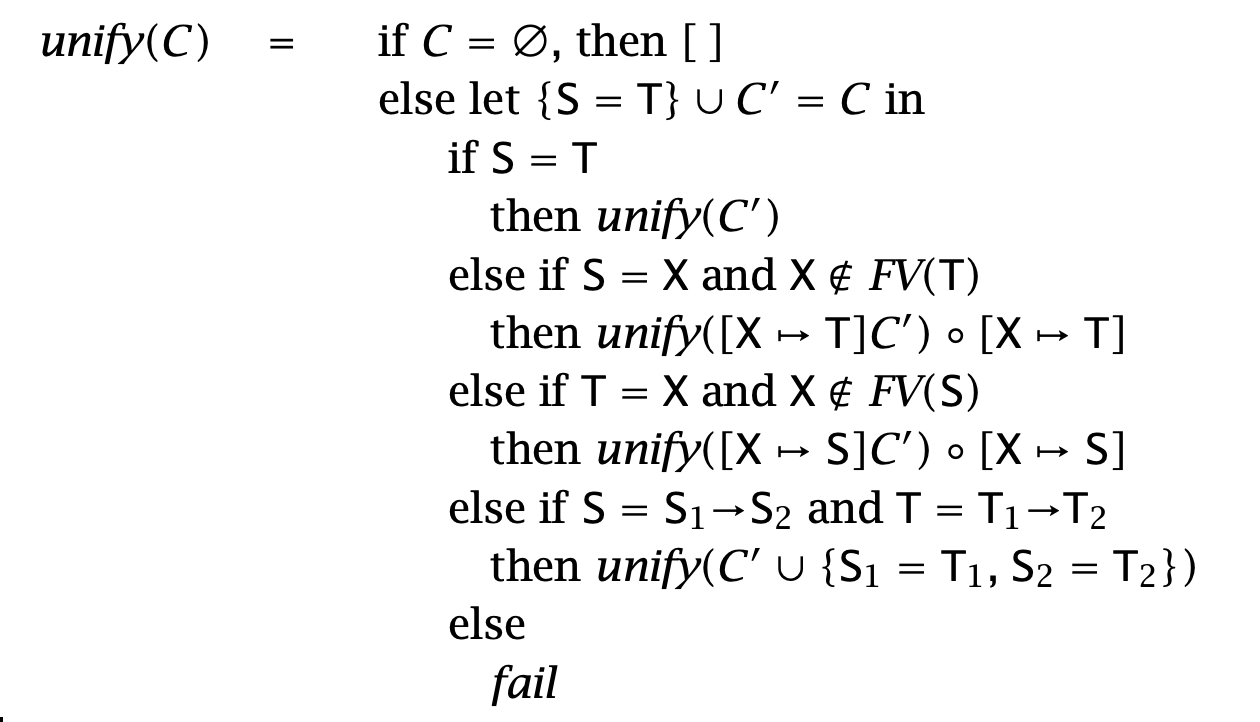
\includegraphics[width=\linewidth]{unification-algorithm.png}

    % featherweight java (wtf?)

    % subtyping
    \subsection{Subtyping}
    $S <: T$ says `$S$ is a subtype of $T$'.\\
    Unlike `subsets' a subtype is `more informative', meaning it may contain more parameters, but never fewer. So a subtype can always be used safely in place of the `supertype.'\\
    e.g. $S = \{x : \text{Nat}, y: \text{Nat}\}, T = \{x : \text{Nat}\}$, so $S <: T$.\\

    \subsubsection{Rules}
    T-Sub: \(\frac{\Gamma \vdash t : S \quad S <: T}{\Gamma \vdash t : T}\)\\
    \textit{`subtype can be typed as its supertype, too'}\\
    S-Refl: \(S <: S\)\\
    \textit{`everything is a subtype of itself'}\\
    S-Trans: \(\frac{S<: U \quad U<:T}{S<:T}\)\\
    \textit{`subtype relation is transitive'}\\
    S-RcdWidth: \(\{ l_{i}: T_{i}^{i \in  1..n +k} \} <: \{ l_{i}: T_{i}^{i \in  1..n} \}\)\\
    \textit{`we can add extra fields in a record, still a subtype'}\\
    S-RcdDepth: \(\frac{\text{for each } i \quad S_{i} <: T_{i}}{\{ l_{i}: S_{i}^{i \in  1..n } \} <: \{ l_{i}: T_{i}^{i \in  1..n} \}}\)\\
    \textit{`can also add depth-wise (within each field's fields)'}\\
    S-RcdPerm: \(\frac{\{k_{j} :S_{j}^{j \in 1..n}\} \text{ is perm. of } \{l_{i}:T_{i}^{i \in 1..n} \}}{\{k_{j}:S_{j}^{j \in 1..n} \} <: \{l_{i}: T_{I}^{i \in 1..n} \}}\)\\
    \textit{`order of fields does not matter (can be a permutation)'}\\
    S-Arrow: \(\frac{T_{1} <: S_{1} \quad S_{2} <: T_{2}}{S_{1} \to S_{2} <: T_{1} \to T_{2}}\)\\
    \textit{`a function that takes in less information and outputs more, is a subtype of a function that takes in more information and outputs less'}\newline

    \textbf{Definition}: $S <: T$ means that an element of S may be safely used whereever an element of T is expected.\\
    This S-Arrow subtype relation is \textbf{contravariant} in the left-hand sides of arrows , and
    \textbf{covariant} in the right-hand sides of arrows.
    The intuition is that if we have a function \(S_1 \to S_2\),
    then it will accept any subtype of \(S_1\) as input,
    and the result \(S_2\) can be viewed as belonging to any supertype of \(S_2\).\\
    S-Top: \(S<: \text{Top}\), where \(\text{Top}\) is a new type constant that is a supertype of every type.\\
    \textbf{Definition:} Liskov's substitution principle: If X inherits from Y, then X should pass
    all of Y's black box texts. Functions that use pointers or references to base classes must be able to use objects of derived classes without knowing it. A function works on all subclasses of a class. \\
    \textbf{Rules:} (1) Inherited methods of a class must not strengthen preconditions or weaken
    postconditions; it must accept a superset of the values the parent method accepts and output a subset
    of the parent’s possible outputs. The parameters must be contravariant and the return values covariant.
    (2) Subtypes must not weaken the class invariants. (3) History rule: the subtype cannot change in a
    way prohibited by the supertype,

    \section{Q\&A}

    \subsection{Q1 Practice Answer}

    % CBN Example
    %((λx.λy.y y)((λw.w w)(λw.w w)))(λw.w)  
    %(λy.y y) (λw.w) - λx is called, all x’s replaced w/ (λw.w w)(λw.w w) 
    %(λw.w) (λw.w) - λy is called, all y’s replaced w/ (λw.w)
    %(λw.w) - λw is called, all w’s replaced w/ (λw.w)
    \subsubsection{CBN}
    \begin{align*}
         & ((\lambda x.\lambda y.y y)((\lambda w.w w)(\lambda w.w w)))(\lambda w.w)      \\
         & \textrm{//\(\lambda x\) is called, all \(x\)'s replaced}                      \\
         & (\lambda y.y y) (\lambda w.w)                                                 \\
         & \textrm{//\(\lambda y\) is called, all \(y\)'s replaced w/ \((\lambda w.w)\)} \\
         & (\lambda w.w) (\lambda w.w)                                                   \\
         & \textrm{//\(\lambda w\) is caled, all \(w\)'s replaced w/ \((\lambda w.w)\)}  \\
         & (\lambda w.w)
    \end{align*}

    %CBV Example
    % (λx.λy.y y)((λw.w w)(λw.w w))(λw.w) 
    %(λx.λy.y y)((λw.w w)(λw.w w))(λw.w) - λw is called, all w’s replaced w/ (λw.w w)
    % Does not terminate, infinite loop of (λw.w w)(λw.w w)
    \subsubsection{CBV}
    \begin{align*}
         & (\lambda x.\lambda y.y y)((\lambda w.w w)(\lambda w.w w))(\lambda w.w) \\
         & (\lambda x.\lambda y.y y)((\lambda w.w w)(\lambda w.w w))(\lambda w.w) \\
         & \textrm{//infinite loop}
    \end{align*}

    \subsection{Q2 - CBV rules given CBN rules for pairs and projections}
    \begin{mathpar}
        \inferrule
        { e_1 \to e_1'}
        { (e_1, e_2) \to (e_1', e_2) }
        \qquad
        \inferrule
        { e_2 \to e_2'}
        { (v_1, e_2) \to (v_1, e_2') }
        \qquad\\
        \inferrule
        { e_1 \to e_1'}
        { \mathrm{fst}\ e_1 \to \mathrm{fst}\ e_1' }
        \qquad
        \inferrule
        { e_1 \to e_1'}
        { \mathrm{snd}\ e_1 \to \mathrm{snd}\ e_1' }
        \qquad\\
        \inferrule
        { }
        { \mathrm{fst}\ (v_1, v_2) \to v_1 }
        \qquad
        \inferrule
        { }
        { \mathrm{snd}\ (v_1, v_2) \to v_2 }
    \end{mathpar}
    CBV requires the full evaluation of the expression under fst/snd before operating on it. This means that the pair fst/snd is operating over must contain two expressions that can be fully evaluated.
    % shoutout elite
    \subsection{Q8 - Expression evaluates in more steps under cbv}
    \begin{flalign*}
         & (\lambda x,y. x x y) ((\lambda x. x) b) ((\lambda x. x) b)                &  & \\
         & \text{under cbn:}                                                         &  & \\
         & (\lambda x,y. x x y) ((\lambda x. x) b) ((\lambda x. x) b)                &  & \\
         & = (\lambda y. ((\lambda x. x) b) ((\lambda x. x) b) y) ((\lambda x. x) b) &  & \\
         & = ((\lambda x. x) b) ((\lambda x. x) b) ((\lambda x. x) b)                &  & \\
         & = b ((\lambda x. x) b) ((\lambda x. x) b)                                 &  & \\
         & \text{under cbv:}                                                         &  & \\
         & (\lambda x,y. x x y) ((\lambda x. x) b) ((\lambda x. x) b)                &  & \\
         & = (\lambda x,y. x x y) b ((\lambda x. x) b)                               &  & \\
         & = (\lambda x,y. x x y) b b                                                &  & \\
         & = (\lambda y. b b y) b                                                    &  & \\
         & = b b b                                                                   &  &
    \end{flalign*}

    \subsection{Q3 - Fix Incoherent Rules}
    \begin{mathpar}
        \inferrule
        { e_1 \to e_1' }
        { \mathrm{and}\ e_1\ e_2 \to \mathrm{and}\ e_1'\ e_2 }
        \qquad
        \inferrule
        { }
        { \mathrm{and}\ \mathrm{true} \ e_2 \to e_2}
        \qquad\\
        \inferrule
        { }
        { \mathrm{and}\ \mathrm{false} \ e_2 \to \mathrm{false}}
    \end{mathpar}
    The first rule is for and checks if $e_1$ can be evaluated. The old rules checked if the second term was true or false, meaning that $e_2$ would have to be the term true or false since there is no rule to evaluate $e_2$ to see if it is true or false.

    % shoutout elite
    \subsection{Q9 - Expression evaluates in more steps under cbn}
    \begin{flalign*}
         & (\lambda x. (\lambda y. y y) x x) (\lambda y. y) x  &  & \\
         & \text{under cbn:}                                   &  & \\
         & = (\lambda y. y y) (\lambda y. y) (\lambda y. y)  x &  & \\
         & = (\lambda y. y) (\lambda y. y) (\lambda y. y)  x   &  & \\
         & = (\lambda y. y) (\lambda y. y)  x                  &  & \\
         & = (\lambda y. y)  x                                 &  & \\
         & = x                                                      \\
         & \text{under cbv:}                                   &  & \\
         & = (\lambda x. (\lambda y. y y) x x) x               &  & \\
         & = (\lambda y. y y) x x                              &  & \\
         & = x x x                                             &  & \\
    \end{flalign*}

    % shoutout bani
    \subsection{Q10 - Expression evaluates in exactly 2 steps under both but then gets stuck}
    \underline{Note 1:} stuck means that a term evaluates to a normal form (no other possible
    eval rules can be applied) but not a value (as defined by bnf usually). \\
    \underline{Note 2:} This solution can be extended for any number of eval steps greater than
    2. Add as many identity functions in between the first two terms as you want to increase the
    number of eval steps by the same amount.
    \begin{flalign*}
         & (\lambda x. x) ((\lambda x. x) z) (\lambda x. x) \\
         & \text{under cbn:}                                \\
         & = ((\lambda x. x) z) (\lambda x. x)              \\
         & = z (\lambda x. x)                               \\
         & \text{under cbv:}                                \\
         & = (\lambda x. x) z (\lambda x. x)                \\
         & = z (\lambda x. x)                               \\
    \end{flalign*}

    \subsection{Q13 - What's the point of an eval strategy?}
    The point of having an evaluation strategy is for you or a computer to know how to evaluate an
    expression if multiple reductions are possible. We need them for building operational semantics. If
    there isnt an eval strategy then evaluating an expression would be nondeterministic.

    \subsection{17 - Convention used with respect to bound variables}
    The convention used is alpha-equivalence. It captures the idea that it's safe to rename a variable in
    a program if you also fix all the references to that variable. That is, when you change the parameter
    of a lambda term, you also have to go into the lambda's body and change the usages of that variable.
    Terms that differ only in the names of bound variables are interchangeable in all context.
    You can change the name of a bound variable in a statement and
    the statements before and after the change are the same. e.g. $(\lambda x.x)$ is alpha equivalent to
    $(\lambda y.y)$.

    \subsection{Question 18 (5) - Unification}
    Unify $a \rightarrow a, \, (b \rightarrow c) \rightarrow (d \rightarrow e), \, \text{and} \,
        (d \rightarrow c) \rightarrow a$.
    \begin{align*}
         & \{a \ra a = (b \ra c) \ra (d \ra e), \, a \ra a = (d \ra c) \ra a \} | []         \\
         & \{a = (b \ra c), \, a = (d \ra e), \, a = (d \ra c), \, a \ra a \} | []           \\
         & \{a = (d \ra e), \, a = (d \ra c) \} | \sigma_1 [a / (b \ra c)]                   \\
         & \{(b \ra c) = (d \ra e), \, (b \ra c) = (d \ra c) \} | \sigma_2 [] \circ \sigma_1 \\
         & \{b = d, \, c = e, \, b = d, \, c = c \} | \sigma_2 [] \circ \sigma_1             \\
         & \{b = d, \, c = e \} | \sigma_2 [] \circ \sigma_1                                 \\
         & \{c = e \} | \sigma_2 [b / d] \circ \sigma_1                                      \\
         & \{c = e \} | \sigma_3 [] \circ \sigma_2 \circ \sigma_1                            \\
         & \{ \} | \sigma_3 [c / e] \circ \sigma_2 \circ \sigma_1                            \\
         & \sigma = [c / e] \circ [b / d] \circ  [a / (b \ra c)]
    \end{align*}

    \subsection{Question 19}
    \begin{enumerate}
        \item{
              \begin{flalign*}
                   & h :: (a \ra a \ra b) \ra a \ra b &  & \\
                   & h \ f \ x = f \ x \ x            &  &
              \end{flalign*}
              }
        \item{
              \begin{flalign*}
                   & c :: (a \ra b) \ra (b \ra c) \ra (a \ra c) &  & \\
                   & c \ f \ g = \backslash x \ra g \ (f \ x)   &  &
              \end{flalign*}
              }
        \item{
              \begin{flalign*}
                   & d :: (a \ra b) \ra (a \ra b \ra c) \ra (a \ra c) &  & \\
                   & d \ f \ g = \backslash x \ra g \ x \ (f \ x)     &  &
              \end{flalign*}
              }
        \item{
              \begin{flalign*}
                   & l \ f = \text{let} \ g \ h \ x = h \ (h \ x) \ \text{in} \ g \ f &  & \\
                   & x :: a                                                           &  & \\
                   & h :: a \ra a                                                     &  & \\
                   & g :: (a \ra a) \ra a \ra a                                       &  & \\
                   & l :: (a \ra a) \ra a \ra a                                       &  &
              \end{flalign*}
              }
    \end{enumerate}

    \subsection{Question 23}
    Why are the semantics of case-of (for sums) in a CbV language weird? Why is this inevitable? Why are the semantics fine in CbN? Contrast this with `either` in Haskell.\\
    In CbV we would expect to evaluate the inside fully before the outside. However, this is again not the case, as we first evaluate the case statement, before deciding where to substitute it. This is inevitable, as for sum types, the valid evaluation steps changes based on the specific type we are dealing with.\\
    In CbN we do not evaluate the argument before passing it to begin with, so it is as one would expect.\\
    % Is either supposed to be different???

    \section{Miscellaneous}
    \textbf{Y-combinator:} $(\lambda x. x x)$ \\
    \textbf{$\Omega$-combinator:} $(\lambda x. x x) (\lambda x. x x)$
\end{multicols*}

\end{document}
